\documentclass[12pt]{article}
\usepackage[utf8]{inputenc}
\usepackage{graphicx}
\usepackage[T1]{fontenc}
\title{Tarea 4 métodos computacionales}



\begin{document}

\author{Humberto Ariza}


\begin{abstract}
    Métodos Computacionales
    Tarea 4 — 2018–20
\end{abstract}

\section{ODE}

\begin{figure}
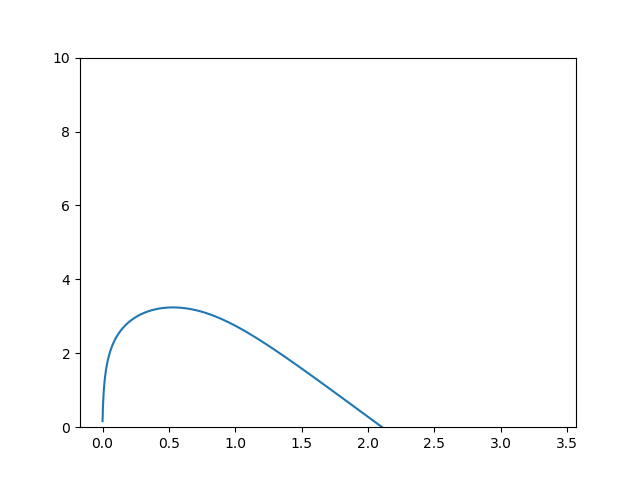
\includegraphics{ODES45.png}
\caption{ODES con 45}
\end{figure}

Como es posible observar el método no estabiliza correctamente. 

\begin{figure}
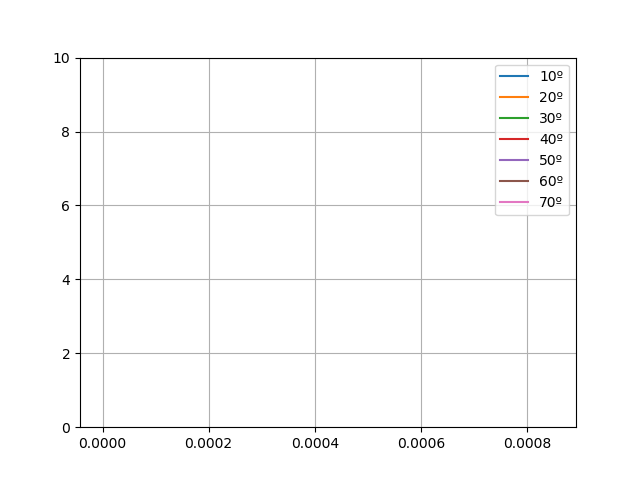
\includegraphics{ODESANGULOS.png}
\caption{ODE CON DIFERENTES ANGULOS}
\end{figure}
Este método debería realizar el recorrido más largo con 20 grados , sin embargo no es lo que se observa en la gráfica obtenida por runge kutta 4.


\section{PDE}

\end{document}